\documentclass[a4paper,11pt]{article}
\usepackage[T1]{fontenc}
\usepackage[utf8]{inputenc}
\usepackage[francais]{babel}
\usepackage{lmodern}
\usepackage{amsmath}
\usepackage{graphicx}
\setlength\abovecaptionskip{0.10ex}
\RequirePackage{graphicx}
\DeclareGraphicsExtensions{.pdf,.jpg,.png,.JPG}
\RequirePackage{float}
\usepackage{titling}
\setlength{\droptitle}{-4cm}
\usepackage{fullpage}

\newcommand{\InsertFig}[1]{
\begin{figure}[H]
\begin{center}
\includegraphics[width=.75\textwidth]{img/#1}
\end{center}
\end{figure}}

\newcommand{\InsertFigTitle}[2]{
\begin{figure}[H]
\caption{#2}
\begin{center}
\includegraphics[width=.75\textwidth]{img/#1}
\end{center}
\end{figure}}


\title{Rapport SY09 TP01 - Statistique descriptive, analyse en composantes principales}
\author{Jean-Baptiste Audibert \& Yueqing Qin}
\date{\today} 

\begin{document}
\maketitle

\section{Statistique descriptive} 

\subsection{Données babies}

\noindent Dans cette première partie du TP, on étudie des données sur des bébés (\textit{ 1236 échantillons et 23 variables, cependant nous ne réaliserons l'étude qu'avec 9 variables}). Le but est d'étudier les différentes influences du fait que la mère soit fumeuse ou non sur des caractéristiques du bébé et de la grossesse, mais également sur la mère.
\noindent Nous étudions tout d'abord la différence de poids entre les bébés nés de mères fumeuses et de mères non fumeuses.

\noindent En étudiant le poids des bébés des échantillons, en distinguant les mères fumeuses et non fumeuses , on observe que la moyenne du poids est plus élevé pour une mère fumeuse que non fumeuse : 

\InsertFigTitle{poidsBebesFumeurs}{Résumé des données concernant le poids des bébés à la naissance - mère fumeuse}

\InsertFigTitle{poidsBebesNonFumeurs}{Résumé des données concernant le poids des bébés à la naissance - mère non fumeuse}

\noindent De plus, nous utilisons la représentation en \textit{boite à moustaches} afin d'observer la répartition des valeurs, la dispersion des données mais également la matérialisation de de l'intervalle de confiance de la médiane :  

\begin{figure}[H]
\begin{center}
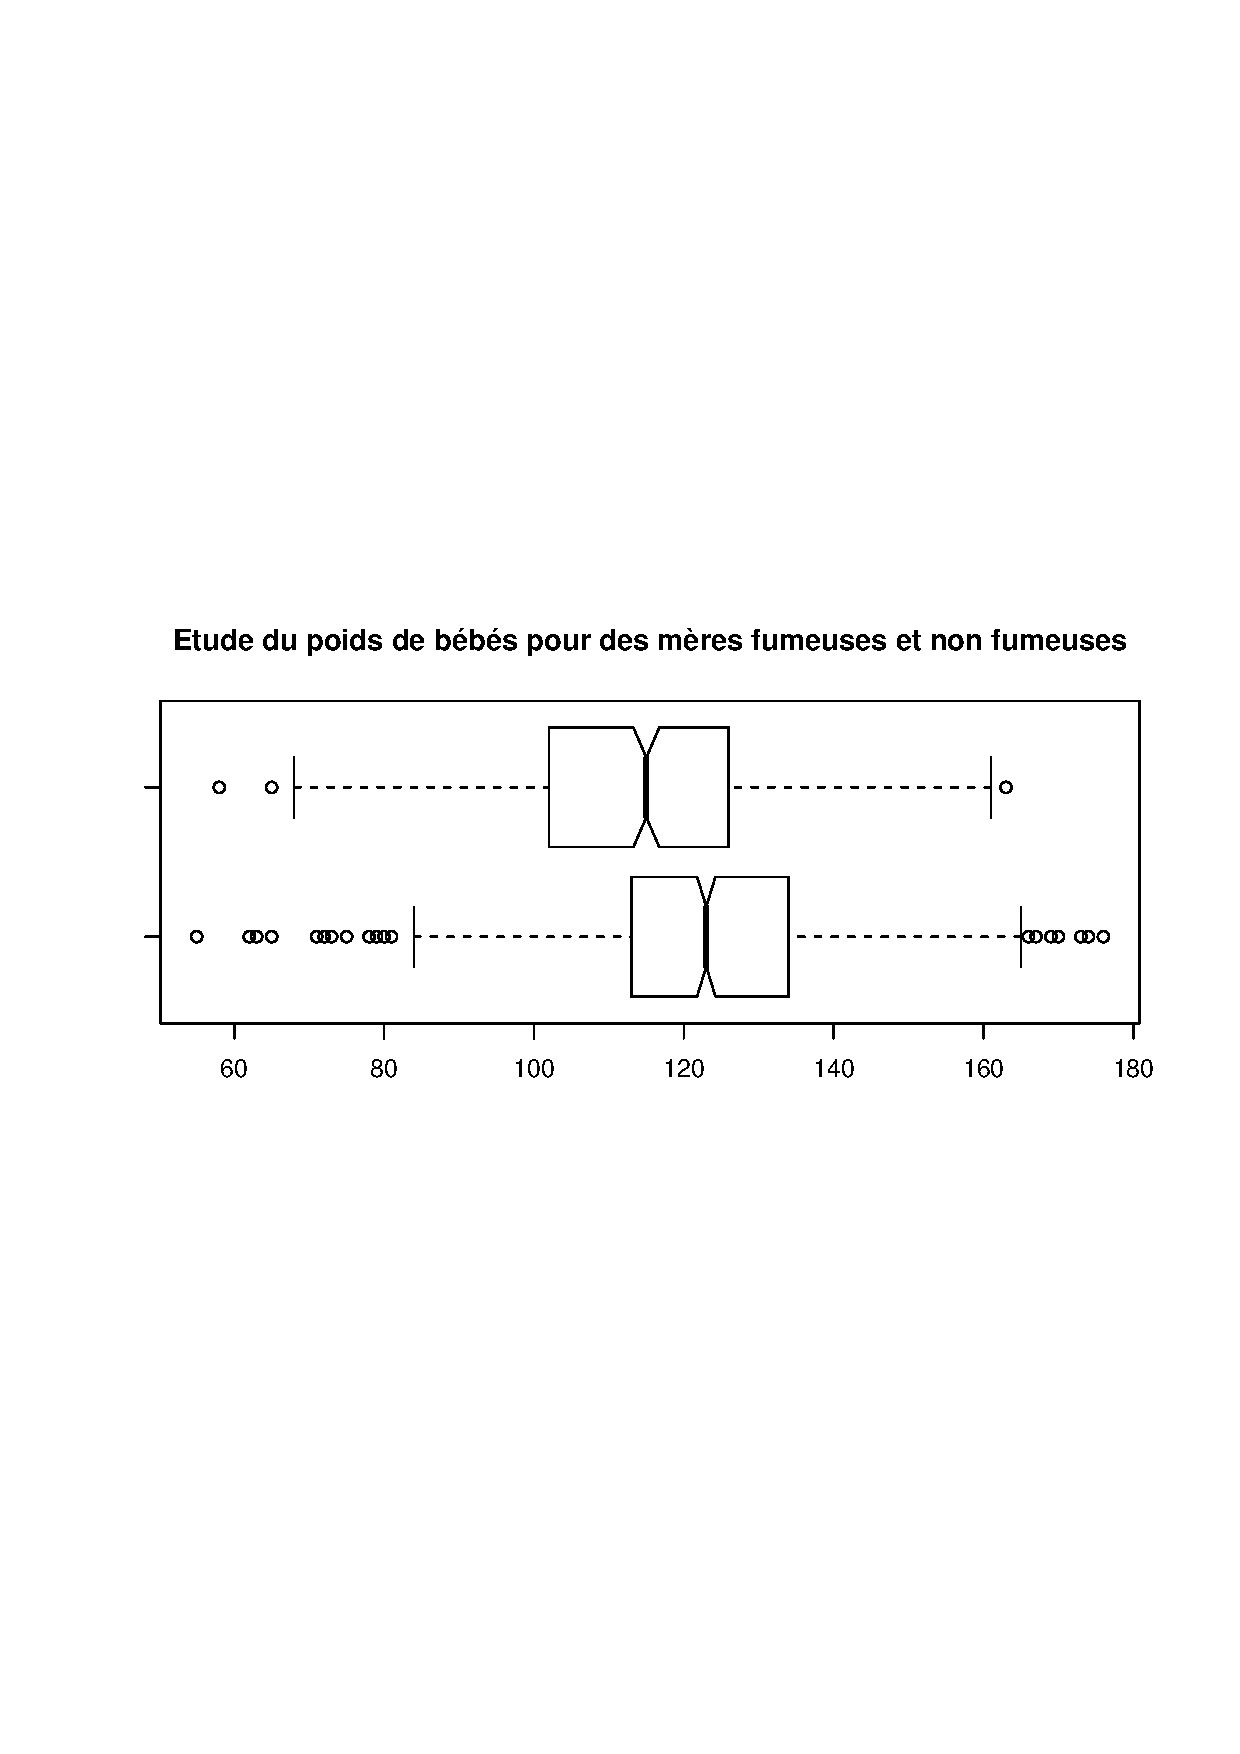
\includegraphics[width=.7\textwidth]{img/poidsbb.jpg}
\end{center}
\end{figure}

\noindent On retrouve en haut la représentation pour une mère non fumeuse, et en bas celle pour une mère non fumeuse. On observe d'emblée que la répartition des valeurs est très différente selon que la mère soit fumeuse ou non. De plus, on observe que les intervalles de confiance de la médiane sont disjoints, ce que nous permet de confirmer R : soit $m_f$ la médiane pour une mère fumeuse et $m_{nf}$ la médiane pour une mère non fumeuse, on a $m_f \in [121.8;124.2]$ et ${m_nf} \in [113.3;116.7]$, soit $IC_{m_f} \cap IC_{ m_nf} = \emptyset$. D'après cela, on peut dire que le fait que la mère soit fumeuse a bien une influence sur le poids du bébé à la naissance. \\

\noindent On s'intéresse maintenant au temps de gestation de la mère, selon qu'elle soit fumeuse ou non.  

\InsertFigTitle{gestationmerefumeuse}{Résumé des données concernant le temps de gestation - mère fumeuse}

\InsertFigTitle{gestationmerenonfumeuse}{Résumé des données concernant le temps de gestation - mère non fumeuse}

\noindent On observe également une différence dans la moyenne, cependant elle parait très peu significative puisque égale à $0.79\%$ Etudions l'affichage avec les boites à moustache : 

\begin{figure}[H]
\begin{center}
\includegraphics[width=.6\textwidth]{img/tempsgestation}
\end{center}
\end{figure}

\noindent Ce que l'on pensait est ici confirmé, les intervalles de confiance de la médiane ne sont pas disjoints ( $m_{nf} \in [280.05;281.93]$ et $m_f \in [277.92;280.08]$, d'où $IC_{m_f} \cap IC_{ m_nf} \ne0$). Ainsi, on peut dire que le fait que la mère soit fumeuse n'influe pas sur le temps de gestation. \\

\noindent On s'intéresse enfin à la corrélation entre le fait que la mère soit fumeuse et le niveau d'étude. Pour cela, on utilise un tableau de contingence, ainsi que son histogramme afin étudier la proportion de mère fumeuse dans chaque \textit{niveau d'étude} : \\

\begin{figure}[H]
\begin{center}
\includegraphics[width=.6\textwidth]{img/histo.jpg}
\end{center}
\end{figure}

\noindent Les échantillons pour des niveaux d'étude 7 et 9 ne sont pas utilisés car les populations sont trop faibles pour être utiles dans l'étude. On observe ici que plus le niveau d'étude est élevé, plus la proportion de mères \textit{non fumeuses} augmente. Ainsi, on peut bien dire que le niveau d'étude a une influence sur le fait que la mère soit fumeuse ou non.

\subsection{Données crabes}

\noindent Nous allons désormais étudier des données morphologiques sur des crabes. L'échantillon est composé de 200 crabes, étudiés avec huit variables. Cependant, nous n'utiliserons que les 5 variables \textit{quantitatives} afin de mener l'étude. \\

\noindent On souhaite tout d'abord s'il est possible de distinguer les caractéristiques morphologiques des crabes selon leur espèce et/ou leur sexe, puis de les identifier en utilisant ces caractéristiques morphologiques.
\noindent Pour cela, on étudie tout d'abord deux graphiques de corrélation entre les variables, selon l'espèce, et le sexe.

\begin{figure}[H]

  \begin{minipage}[b]{0.45\linewidth}
   \centering
   \InsertFig{pairs1.png} 
  \end{minipage}
\hfill
  \begin{minipage}[b]{0.45\linewidth}
   \centering
  \InsertFig{pairs2.png}     
  \end{minipage}

  \caption{Etude des corrélations avec la fonction pairs}
  \label{fig:ma_fig}

\end{figure}

\noindent Les variables sont très corrélées et on ne peut pour l'instant affirmer qu'il y a des différences significatives selon le sexe ou l'espèce. On étudie donc l'influence des variables quantitatives sur les variables qualitatives en  utilisant des représentations en boite à moustache. Nous n'avons pu inclure tous les graphiques dans le rapport, faute de place.

\noindent Toutefois, grâce à ces représentations, et en utilisant les intervalles de confiance sur la médiane, on peut affirmer qu'il y a des différences morphologiques selon l'espèce et le sexe. 

\noindent Nous allons maintenant étudier la corrélation entre les variables. Les calculs nous donnent :

\begin{figure}[H]
\begin{center}
\includegraphics[width=.5\textwidth]{img/corcrabs.png}
\end{center}
\end{figure}

\noindent On observe qu'effectivement, les variables sont très corrélées. Ceci est dû à un phénomène physique simple : quand on est en présence  d'un \textit{petit crabe}, l'ensemble de ses attributs est \textit{petit}, et inversement. Pour supprimer la corrélation, on pourrait diviser par une des variable, à priori la plus corrélée avec les autres, et recommencer l'étude.

\section{Analyse en composante principale}

\subsection{Exercice théorique}

\subsubsection{Axes factoriels et pourcentages d'inertie expliquée}
\noindent Matrice des valeurs propres / axes factoriels : 
\begin{center}
$ \begin{pmatrix}
0&0&1\\
-0.707&0.707&0\\
0.707&0.707&0
\end{pmatrix}$
\end{center}

\noindent Pourcentage d'inertie expliqué par chacun des axes : $57.14 \%$, $28.57 \%$, $14.59 \%$. Le troisième axe est donc clairement le moins intéressant pour l'étude. 

\subsubsection{Composantes principales et représentation dans le premier plan factoriel}

\noindent Matrice des composantes principales : 
\begin{center}
$ \begin{pmatrix}
-1.414&2.220*10^{-16}&1\\
-1.414&2.220*10^{-16}&-1\\
1.414&1.414&0\\
1.414&-1.414&0
\end{pmatrix}$
\end{center}
\noindent Et on représente les individus dans le premier plan factoriel : 
\begin{figure}[H]
\begin{center}
\includegraphics[width=.6\textwidth]{img/premierplanfactoriel}
\end{center}
\end{figure}
 %\InsertFigTitle{premierplanfactoriel}{Représentation des quatre individus dans le premier plan factoriel}

\subsubsection{Représentation des 3 variables dans le premier plan factoriel}

\begin{figure}[H]
\begin{center}
\includegraphics[width=.6\textwidth]{img/ppf}
\end{center}
\end{figure}

\subsubsection{Calcul de reconstitution} 

\paragraph{$k=1$}

\begin{center}$\displaystyle\sum_{\alpha =1}^{1} c_{\alpha} u_{\alpha}^{t} =$ 
$\begin{pmatrix}
0&1&-1\\
0&1&-1\\
0&-1&1\\
0&-1&1
\end{pmatrix}$
\end{center}

\paragraph{$k=2$}

\begin{center} $\displaystyle\sum_{\alpha =1}^{2} c_{\alpha} u_{\alpha}^{t} = $
$\begin{pmatrix}
0&1&-1\\
0&1&-1\\
0&0&2\\
0&-2&0
\end{pmatrix}$
\end{center}

\paragraph{$k=3$}

\begin{center} $\displaystyle\sum_{\alpha =1}^{3} c_{\alpha} u_{\alpha}^{t} = $
$\begin{pmatrix}
1&1&-1\\
-1&1&-1\\
0&0&2\\
0&-2&0
\end{pmatrix}$
\end{center}

\subsection{Utilisation des outils R}
\subsubsection{Reprise des résultats}


%\noindent Matrice de départ :
%\begin{center}
%$ \begin{pmatrix}
%6.0&6.0&5.0&5.5&8\\
%8.0&8.0&8.0&8.0&9\\
%6.0&7.0&11.0& 9.5&11\\
%14.5&14.5&15.5&15.0&8\\
%14.0&14.0&12.0&12.5&10\\
%11.0&10.0&5.5&7.0&13\\
%5.5&7.0&14.0&11.5&10\\
%13.0&12.5&8.5&9.5&12\\
%9.0&9.5&12.5&12.0&18
%\end{pmatrix}$
%\end{center} 

\noindent On reprend l'exemple du cours, avec les différentes fonctions fournies par \textbf{R}.

\noindent Avec l'appel \textit{acp <- princomp(A)}, où A est la matrice de départ, on obtient l'ensemble des résultats dans l'objet \textit{acp}. On obtient ainsi par exemple la matrice des vecteurs propres, ou la mtrice des composantes principales : 

\begin{figure}[H]

  \begin{minipage}[b]{0.45\linewidth}
   \centering
   \InsertFig{acp$loadings} 
  \end{minipage}
\hfill
  \begin{minipage}[b]{0.45\linewidth}
   \centering
  \InsertFig{acp$scores.png}     
  \end{minipage}

  \caption{Affichage de résultats de la fonction princomp : matrice des vecteurs propres et matrice des composantes principales}
  \label{fig:ma_fig}
  \end{figure}
  
  \noindent Avec la fonction plot classique, on obtient la projection des individus dans le premier axe factoriel : 
  
\begin{figure}[H]
\begin{center}
\includegraphics[width=.7\textwidth]{img/acp1.png}
\end{center}
\end{figure}

\subsubsection{Fonction princomp, plot et biplot}

\noindent La fonction \textbf{plot} affiche la variance des différents composants. Une variance élevée est intéressante pour effectuer l'analyse. En effet, la variance est égale à la valeur de propre de la composante.
\noindent La fonction \textbf{biplot} affiche la représentation des individus dans les deux principaux axes d'inertie. Elle affiche également les vecteurs de corrélation entre les variables.

\begin{figure}[H]

  \begin{minipage}[b]{0.45\linewidth}
   \centering
   \InsertFig{plotacp} 
  \end{minipage}
\hfill
  \begin{minipage}[b]{0.45\linewidth}
   \centering
  \InsertFig{biplotacp}     
  \end{minipage}

  \caption{Affichage de résultats des fonctions plot et biplot pour l'ACP}
  \label{fig:ma_fig}
  
  \end{figure}
  
\subsection{Traitement des données Crabs par l'ACP}

\subsubsection{Première analyse sans traitement préalable}

\noindent Nous allons désormais appliquer l'ACP sur les données \textbf{Crabs}, afin d'étudier les données et d'essayer d'identifier des groupes.
\noindent On effectue tout d'abord l'ACP sans traitement préalable. Avec le \textit{biplot}, on obtient le nuage de points suivants : 

\begin{figure}[H]
\begin{center}
\includegraphics[width=.6\textwidth]{img/acpcrabs.png}
\end{center}
\end{figure}

\noindent On constate qu'il est impossible de distinguer des groupes, selon le sexe ou l'espèce. 

\subsection{Traitement des données Crabs avec traitement préalable}

\noindent On a observé précédemment qu'il était impossible de distinguer des groupes. Ceci est du à un effet de taille, et au fait que les variables sont toutes liés. On va donc chercher à supprimer une variable, afin d'obtenir des données plus promptes à l'analyse. En étudiant les corrélations, on se rend compte que la variable \textbf{CL} est la plus corrélée avec les autres. De plus, avec l'histogramme obtenu par le \textit{plot} de la fonction \textit{princomp}, on se rend compte qu'elle est clairement dominante. \\

\begin{figure}[H]
\begin{center}
\includegraphics[width=.6\textwidth]{img/sumcolcrabs.png}
\end{center}
\end{figure}

\noindent Nous allons donc \textit{supprimer} cette variable en divisant chaque ligne $i$ par la valeur $CL_i$ correspondante, et étudier le jeu de données ainsi obtenus.


\noindent On observe désormais qu'il n'y a plus de variables dominantes comme précédemment. Nous allons projeter dans le premier axe factoriel afin de savoir s'il est possible d'observer distinctement un ou plusieurs groupes : 

\begin{figure}[H]
\begin{center}
\includegraphics[width=.6\textwidth]{img/acpcrabscool1}
\end{center}
\end{figure}

\noindent On observe bien des groupes, cependant, il est difficile de les identifier. Nous allons donc construire quatre groupes avec l'outil \textit{class} de R : MB/MO/FM/FB, correspondant aux différentes associations sexe/espèce. Afin d'afficher ces groupes, on utilise la fonction \textit{xyplot}, du package \textit{lattice}. On obtient le résultat suivant : 

\begin{figure}[H]
\begin{center}
\includegraphics[width=.7\textwidth]{img/acpcool}
\end{center}
\end{figure}

\noindent On peut désormais observer quatre groupes distincts, et donc identifier les crabes.


 







\end{document}